\chapter{Fundamentals}
\label{chap:refs}

A main advantage of ray tracing algorithms is that the core procedure is not complicated when viewed from a theoretical point of view. Figure \ref{fig:raytracer_general} shows an example of a virtual scene. It consists of an orange sphere, a white ground plane and a plane acting as an area light source. Furthermore, there exists an image plane on which the 2D image of the 3D scene will be projected. 

\begin{figure}[h]
	\centering
	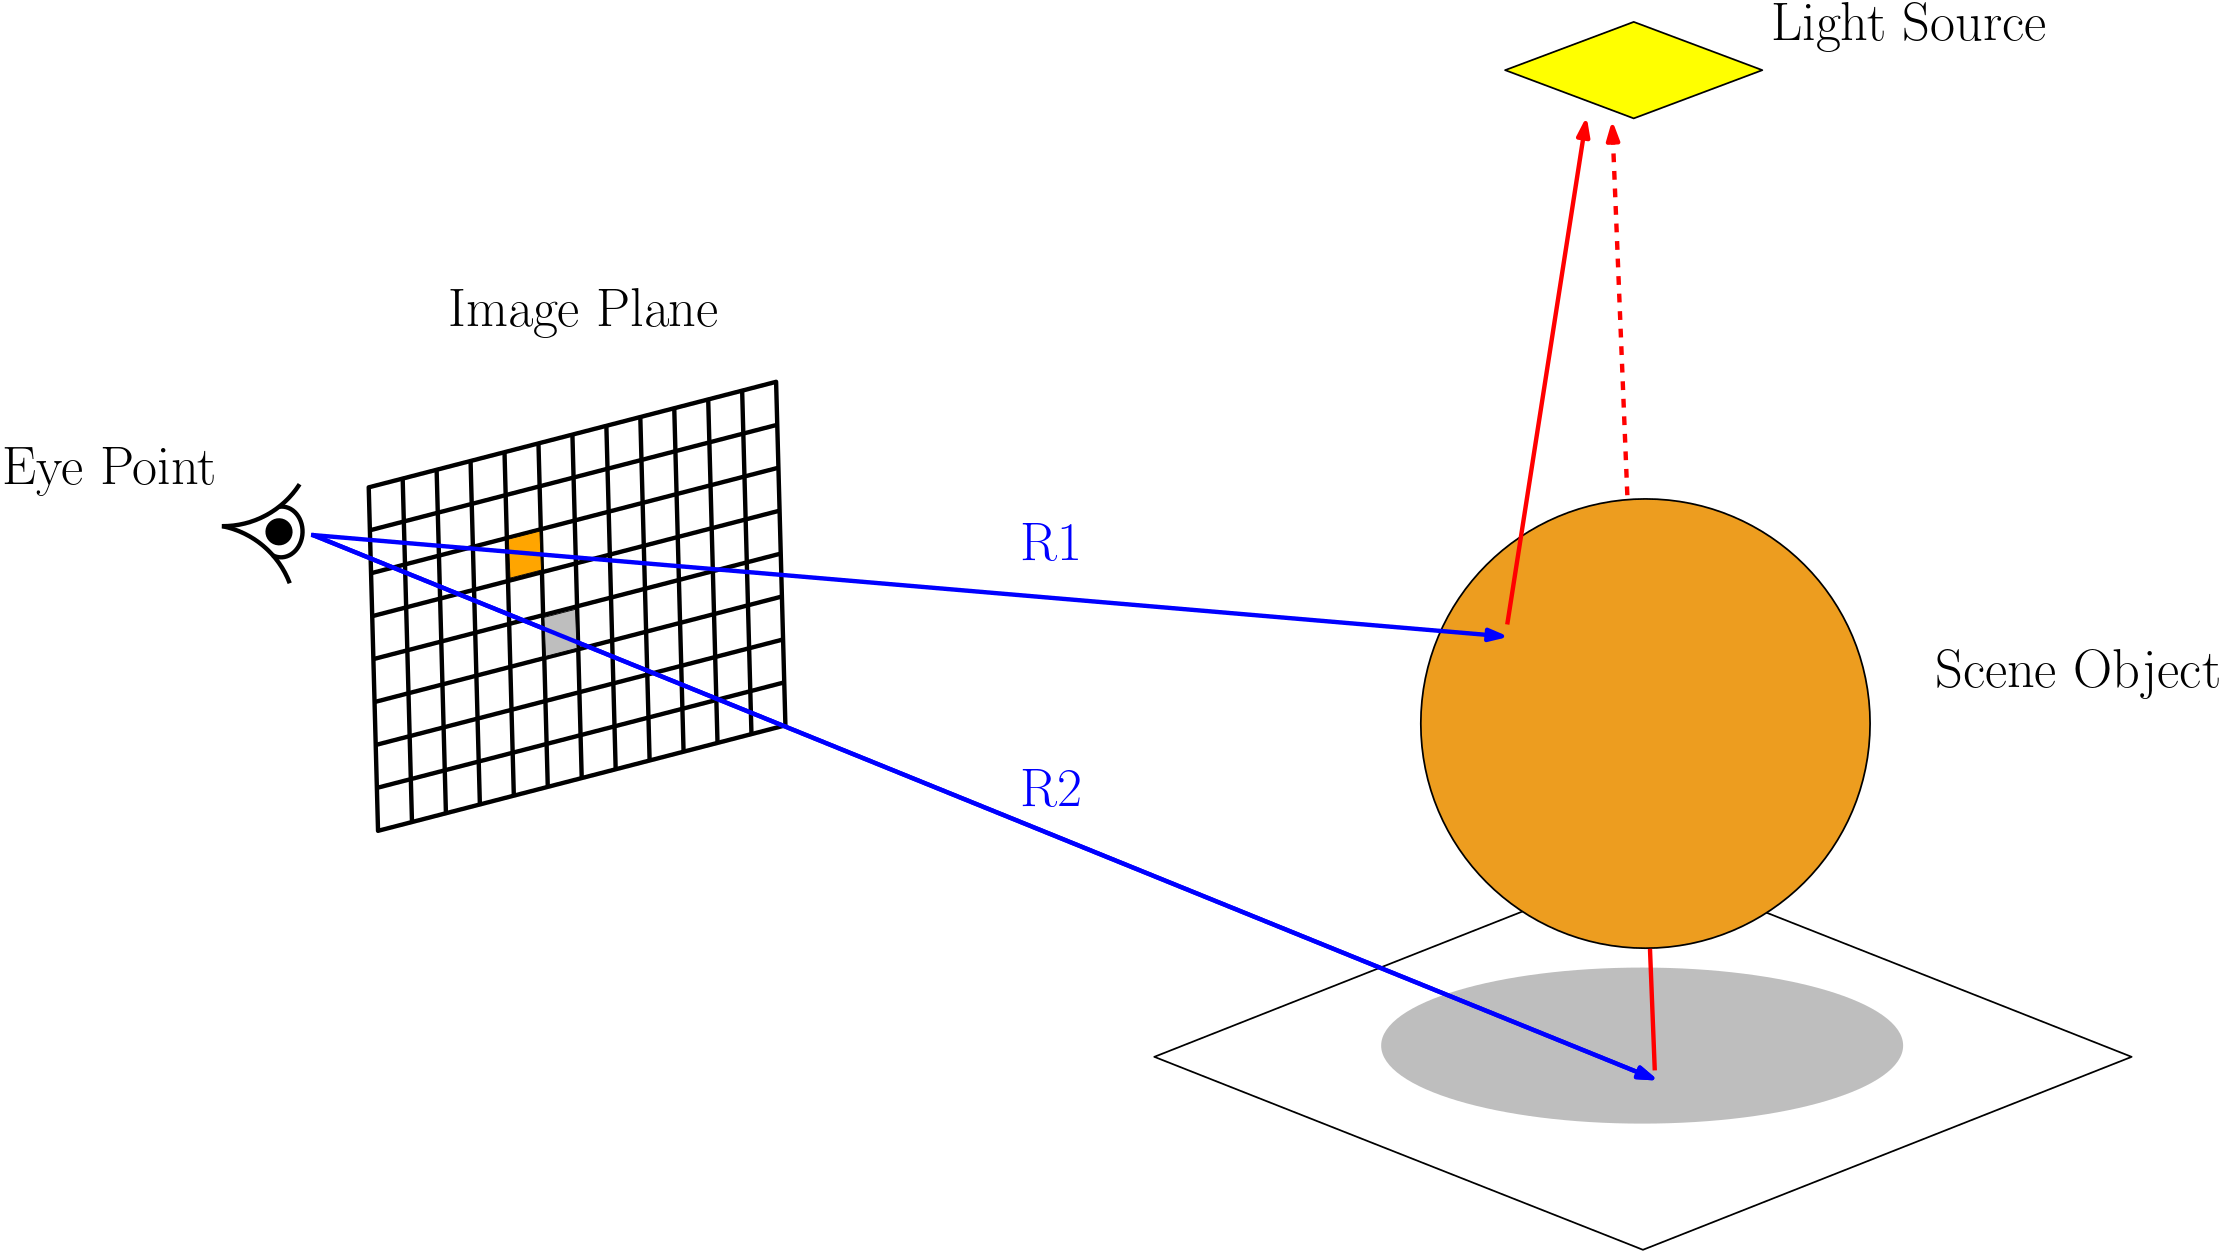
\includegraphics[width=.9\linewidth]{img/1 fundamentals/ray_tracing.png}
	\caption{Ray tracing procedure for calculating global illuminate.}
	\label{fig:raytracer_general}
\end{figure}

This projection done via casting of rays. A ray is a [something] consisting of two components. An origin point and a direction vector. The "Eye Point" in \ref{fig:raytracer_general} will serve as the origin of the cast rays (sometimes, the Eye Point is referred to as Camera or Virtual Camera). In the figure, the image plane consists of multiple "cells", that represents the actual pixels of the resulting image. From each of these cells, a ray is cast into the scene. The next step is to determine, whether that ray hit a geometry by performing intersection testing on all geometries. In case a geometry is hit, a secondary ray is generated with its origin at the intersection point and whose direction is toward the light source. In case there is no geometry in the way between the first intersection point and the light source, this means that the first intersection point is exposed to light and the material color at that point is used for that pixel (see R1 in figure \ref{fig:raytracer_general}). Otherwise the intersection point must be in shadow (see R2). This procedure generates an image with local illumination.

\section{Ray Tracing Techniques}
As briefly mentioned in the Introduction, ray tracing was pioneered in 1968 by \cite{appel1968some}. The aim of this paper was to provide basic shading for line drawings for a better communication of spatial relation and depth of objects.

\begin{figure}[h]
	\centering
	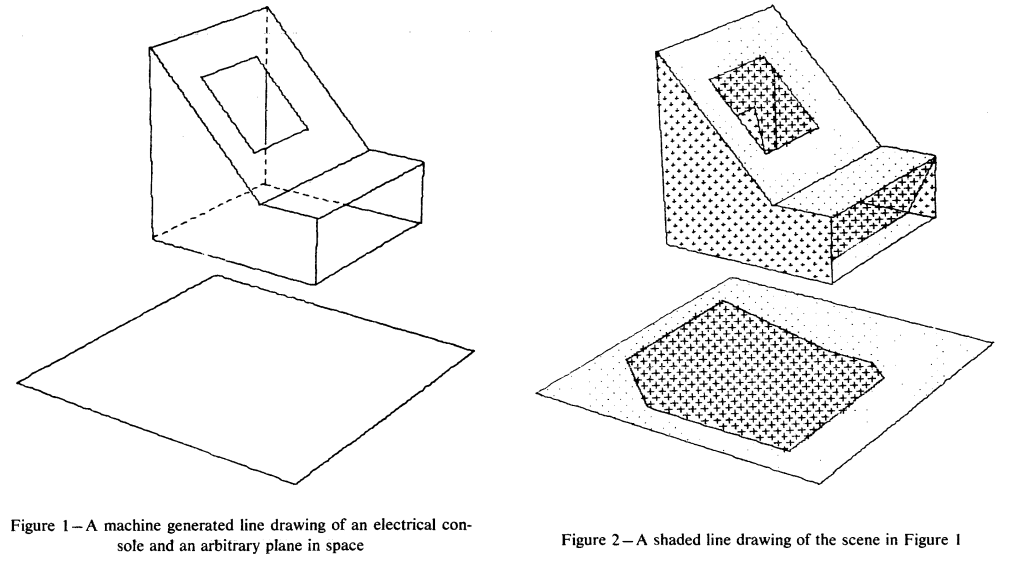
\includegraphics[width=1\linewidth]{img/1 fundamentals/appel_comp}
	\caption{Figures from \cite{appel1968some}. Left figure shows plain solid geometry and right figure shows the same solid with shading applied to it.}
	\label{fig:appel}
\end{figure}

Figure \ref{fig:appel} demonstrates this: without the additional shading information, the observer would have no idea about the position of the upper geometry relative to the plane.
To achieve this shading, virtual light rays are shot from a scene light source in random directions. Whenever one such ray intersects a geometry, a character or symbol (e.g. a "plus"-symbol or small square) is placed at that intersection point. If enough such rays would be cast, areas which are exposed to light would be approximated. The result would then come to be by inverting the shaded and non-shaded areas of the geometry.

The intensity of light incident to the light source is described by the following equation:

\begin{equation}
I = S\frac{\cos{\theta}}{{D}^2}
\end{equation}

where $S$ is the intensity of the light source, $\cos{\theta}$ the angle between the ray and the surface normal at the intersection point and $D$ the distance between intersection point and light source.

In order to achieve convincing results, a high number of rays had to be generated ("Even for about 1000 light rays results were splotchy." \cite[p 3]{appel1968some}). At the time of publication, computational power of hardware could hardly be used for this.

The idea of casting rays later became a key utilization for a shading model that aimed for higher realism by taking the "global setting" of geometries into account \cite{whitted1979improved}. A number of shading systems already existed, that focused on the convincing display of single optical effects. Some models were good at calculating reflection (e.g. the Phong-Shading model \cite{phong1975illumination}), but at the same time could not handle refraction effect. And vice versa. Whitted aimed at unifying the calculations of these shaders. 
In the model which he described and which is shown in Figure \ref{fig:whitted_model}, the light intensity $I$ arriving at the eye point from the intersection point $x$ is conglomerated by the specular reflection $S$ and transmition 

\begin{equation}
I = I_{a} + k_{d} \sum_{j=1}^{j=ls}(N*L_{j}) + k_{d} \sum_{j=1}^{j=ls}(N*L_{j}\prime)^n
\end{equation}

\begin{figure}[h]
	\centering
	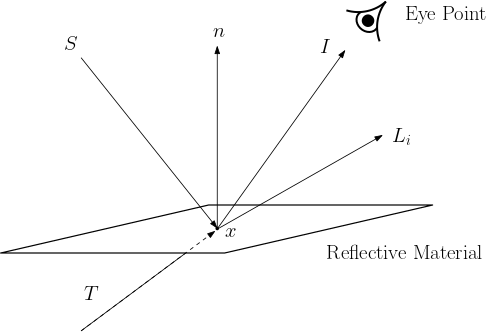
\includegraphics[width=.7\linewidth]{img/1 fundamentals/whitted.png}
	\caption{Shading model of \cite{whitted1979improved}}
	\label{fig:whitted_model}
\end{figure}


\begin{equation}
I = S \sum_{j=1}^{ls} (N*L_{j}) + k_{s}S + k_{t}T
\end{equation}

where S is the light intensity, blah blah.


\begin{equation}
I(x,x\prime) = g(x,x\prime) \left[ e(x,x\prime) + \int_S p(x,x\prime,x\prime\prime)I(x\prime,x\prime\prime) dx\prime\prime \right] 
\end{equation}


\begin{figure}[h]
	\centering
	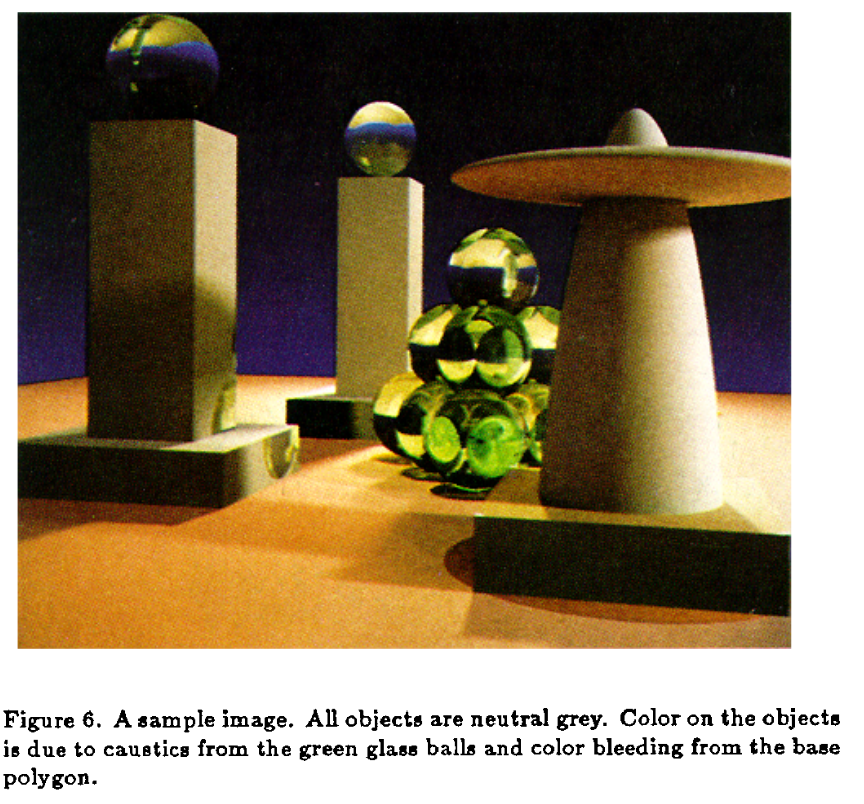
\includegraphics[width=.75\linewidth]{img/1 fundamentals/rendering_eq_figure.png}
	\caption{Figure from \cite{kajiya1986rendering} displaying a scene rendered with his approach.}
	\label{fig:rendering_eq}
\end{figure}


\section{Constructive Solid Geometry}


\section{Limitations}




% new section
\section{Common ray acceleration data structures}
The computational cost associated with ray tracing algorithms has always been regarded as a "necessary evil" one has to face when desiring highly realistic images. An often cited fact is Whitted's observation, that, for complex scenes, 95 percent of the time used by the algorithm is spend on intersection calculations \cite[p 349]{whitted1979improved}. The image displayed in figure \ref{fig:rendering_eq}, was rendered with a resolution of 512 by 512 pixels and with 40 paths per pixel on an IBM 3081 machine consumed during 1221 minutes \cite[p 149]{kajiya1986rendering}. 

It was a logical consequence, that, over time, new ideas were introduced for accelerating the ray tracing process, mostly by minimizing the number of intersection tests. Nowadays, there exist various ray acceleration structures. In the following, two of these structures are that are commonly used, namely bounding volume hierarchies and binary space partitioning trees are introduced.

\subsection{Bounding volume hierarchy}

\subsection{Binary space partitioning}


\section{Intel\textregistered's Embree Framework}
Embree is a high performance rendering framework, consisting of a collection of kernels and data structures suited for the communication with [insert hardware types]. The latest version of Embree at the time of writing this thesis is 3.13.0.